%
% grad.tex
%
% (c) 2021 Prof Dr Andreas Müller, OST Ostschweizer Fachhochschule
%
\begin{frame}[t]
\frametitle{Grad}
\vspace{-20pt}
\begin{columns}[t,onlytextwidth]
\begin{column}{0.48\textwidth}
\begin{center}
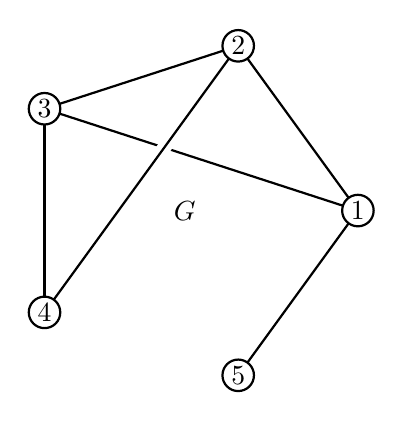
\begin{tikzpicture}[>=latex,thick]

\def\r{2.2}

\coordinate (A) at ({\r*cos(0*72)},{\r*sin(0*72)});
\coordinate (B) at ({\r*cos(1*72)},{\r*sin(1*72)});
\coordinate (C) at ({\r*cos(2*72)},{\r*sin(2*72)});
\coordinate (D) at ({\r*cos(3*72)},{\r*sin(3*72)});
\coordinate (E) at ({\r*cos(4*72)},{\r*sin(4*72)});

\draw[shorten >= 0.2cm,shorten <= 0.2cm] (A) -- (C);
\draw[color=white,line width=5pt] (B) -- (D);
\draw[shorten >= 0.2cm,shorten <= 0.2cm] (B) -- (D);

\draw[shorten >= 0.2cm,shorten <= 0.2cm] (A) -- (B);
\draw[shorten >= 0.2cm,shorten <= 0.2cm] (B) -- (C);
\draw[shorten >= 0.2cm,shorten <= 0.2cm] (C) -- (D);
%\draw[shorten >= 0.2cm,shorten <= 0.2cm] (D) -- (E);
\draw[shorten >= 0.2cm,shorten <= 0.2cm] (E) -- (A);

\draw (A) circle[radius=0.2];
\draw (B) circle[radius=0.2];
\draw (C) circle[radius=0.2];
\draw (D) circle[radius=0.2];
\draw (E) circle[radius=0.2];

\node at (A) {$1$};
\node at (B) {$2$};
\node at (C) {$3$};
\node at (D) {$4$};
\node at (E) {$5$};
\node at (0,0) {$G$};

%\node at ($0.5*(A)+0.5*(B)-(0.1,0.1)$) [above right] {$\scriptstyle 1$};
%\node at ($0.5*(B)+0.5*(C)+(0.05,-0.07)$) [above left] {$\scriptstyle 2$};
%\node at ($0.5*(C)+0.5*(D)+(0.05,0)$) [left] {$\scriptstyle 3$};
%\node at ($0.5*(D)+0.5*(E)$) [below] {$\scriptstyle 4$};
%\node at ($0.5*(E)+0.5*(A)+(-0.1,0.1)$) [below right] {$\scriptstyle 5$};
%\node at ($0.6*(A)+0.4*(C)$) [above] {$\scriptstyle 6$};
%\node at ($0.4*(B)+0.6*(D)$) [left] {$\scriptstyle 7$};

\end{tikzpicture}
\end{center}
\begin{block}{Definition}
Der Grad
$\deg v$
eines Knotens $v\in V$ ist die Anzahl der Kanten mit Ende in $v$
\end{block}
\end{column}
\begin{column}{0.48\textwidth}
\begin{block}{Gradmatrix}
Diagonalmatrix mit $d_{ii}=\deg v_i$
\[
D(G)
=
\begin{pmatrix}
3&0&0&0&0\\
0&3&0&0&0\\
0&0&3&0&0\\
0&0&0&2&0\\
0&0&0&0&1
\end{pmatrix}
\]
\end{block}
\begin{block}{Satz}
Die Summe der Grade ist gerade:
\[
\sum_{i=1}^n\deg v_i = \operatorname{Spur} D(G) \equiv 0 \mod 2
\]
\end{block}
\end{column}
\end{columns}
\end{frame}
